\documentclass[14pt]{beamer}

\usepackage[brazil]{babel}
\usepackage[utf8]{inputenc}
\usepackage[T1]{fontenc}
\usepackage{helvet}
\usepackage{amsmath}
\usepackage{hyperref}
\usepackage{graphicx}
\usepackage{verbatim}

%% selecionar tema (ver documentação do Beamer para mais temas)
\usetheme{Madrid}
%\usecolortheme{seahorse}
\usecolortheme{default}
\useinnertheme{circles}
\useoutertheme{infolines}

%%remove os simbolos de navegação
\setbeamertemplate{navigation symbols}{}

%% acrescentar "(cont.)" ao títulos de slides com quebras
\setbeamertemplate{frametitle continuation}[from second]

%% rodapé (footlines) customizado
\setbeamertemplate{footline}{\leavevmode%
\begin{beamercolorbox}[wd=.33\paperwidth,left,ht=2.5ex,dp=1.5ex,rightskip=4pt
  plus 1pt, leftskip=4pt]{subsection in head/foot}
  \insertshortauthor
\end{beamercolorbox}%
\begin{beamercolorbox}[wd=.33\paperwidth,center,ht=2.5ex,dp=1.5ex]{section in head/foot}
  \usebeamercolor[fg]{section in foot/head}\insertshorttitle
\end{beamercolorbox}%
\begin{beamercolorbox}[wd=.34\paperwidth,ht=2.5ex,dp=1.5ex,leftskip=4pt plus 1pt,rightskip=4pt plus 1pt]{subsection in head/foot}
%   \insertshortdate\hfill\insertframenumber/\inserttotalframenumber %% com a data
%   \hfill\insertframenumber/\inserttotalframenumber %% com o n.o total de slides
   \hfill\insertframenumber
\end{beamercolorbox}%
}

\title{Introdução ao \LaTeX}
\author{Péricles S. da C. Jr. (CRI-STI/UFBA)}
\date{\small Atualizado em \today}

\AtBeginSubsection[]
{
\begin{frame}<beamer>
\frametitle{Agenda}
\tableofcontents[currentsection,currentsubsection]
\end{frame}
}

\begin{document}

\begin{frame}
  \maketitle
\end{frame}

\begin{frame}
  \frametitle{Agenda}
  \tableofcontents
\end{frame}

\section{Contextualização}

\subsection{Histórico}

\begin{frame}
  \frametitle{Donald Knuth}
  \begin{columns}
      \begin{column}{0.6\textwidth}
        \begin{itemize}
          \item <2-> Professor Emérito de Stanford;
          \item <3-> "The Art of Computer Programming";
          \item <4-> Projeto \TeX;
          \item <5-> Desenvolvimento de textos com alta qualidade;
          \item <6-> Em português pronuncia-se "téc", de técnico.          
        \end{itemize}
      \end{column}
      \begin{column}{0.4\textwidth}
        \begin{figure}
          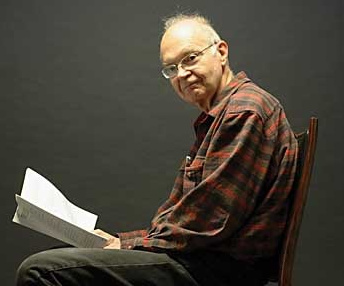
\includegraphics[width=0.9\textwidth]{img/knuth.jpeg}
          \caption{Knuth}
        \end{figure}
      \end{column}
  \end{columns}

\end{frame}

\begin{frame}
  \frametitle{Leslie Lamport}
  \begin{columns}
      \begin{column}{0.7\textwidth}
        \begin{itemize}
          \item <2-> Pesquisador;
          \item <3-> Empregado na Micro\$oft Research;
          \item <4-> Projeto \LaTeX~a partir do \TeX;
          \item <5-> Conjunto de macros de alto nível;
          \item <6-> Baseado em classes
          \item <7-> \textbf{WYSIWYM} - \small{What You See is What You Mean}           
        \end{itemize}
      \end{column}
      \begin{column}{0.3\textwidth}
        \begin{figure}
          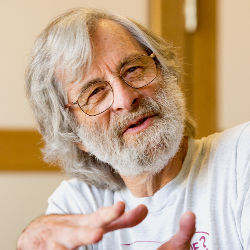
\includegraphics[width=0.9\textwidth]{img/l-lamport.jpg}
          \caption{L. Lamport}
        \end{figure}
      \end{column}
  \end{columns}

\end{frame}

\begin{frame}
  \frametitle{Observações}
  
  \begin{itemize}
    \item <1-> \LaTeX~é uma linguagem de marcação de texto;
    \item <2-> É case sensitive (Maiúscula $\neq$ Minúscula)
    \item <3-> O programa \TeX~é um compilador que lê um arquivo de entrada (.tex) e produz um arquivo de saída (.dvi ou .pdf);
    \item <4-> Segue regras/ideias de linguagens de programação (declarações e corpo do programa, ligação de bibliotecas, regras de escopo e etc.);
 	  \item <5-> Arquivos .tex são arquivo em ASCII que contém o texto acrescido de comandos ou macros \TeX~e \LaTeX.
  \end{itemize}
  
\end{frame}

\begin{frame}[fragile]{Hello World}
  \verb| % O símbolo "%" |\\ 
  \verb| % indica um comentário e é ignorado| \\ 
  \verb| % Hello World versão 1| \\
  \verb| Ol\’{a}, mundo !| \\
  \verb| \bye| \\
    \begin{block}{Compilando}
      \verb| $tex hello.tex |\\
      \verb| $xdvi hello.dvi |
    \end{block}
\end{frame}

\section{Comandos e estruturas \LaTeX}

\subsection{Comandos}

\begin{frame}
  \frametitle{Comandos}
  
  \begin{itemize}
      \item <1-> Comandos \LaTeX~são normalmente precedidos por "\textbackslash"~e seguidos de 
		parâmetros opcionais (delimitados por "["~e "]") e/ou parâmetros 
		obrigatórios (delimitados por "\{"~e "\}");
      \item <2-> Exceção:
      \item <3-> A regra "\$"~que delimita o ambiente matemático
      \begin{itemize}
        \item <4-> Exemplo: \alert{\$3+2\textbackslash sqrt\{2\}\$}, que produz $3+2\sqrt{2}$
      \end{itemize}
  \end{itemize}

\end{frame}

\subsection{Uso de pacotes}

\begin{frame}
  \frametitle{Uso de pacotes}
  
  \begin{itemize}
    \item <1-> Amplia as funcionalidades do \LaTeX;
    \item <2-> Modularidade;
    \item <3-> Sintaxe:
    \item <4-> \textbackslash usepackage[opções]\{\alert{pacote}\};
  \end{itemize}

\end{frame}

\begin{frame}
  \frametitle{Símbolos Reservados}

  \begin{block}{Símbolos Especiais}
    \begin{itemize}
      \item <1-> Análogo à palavras reservadas em linguagem de programação;
      \item <2-> \$ \& \% \# \_ \{ \}
      \item <3-> Para serem obtidos:
      \item <4-> \textbackslash símbolo
    \end{itemize}
  \end{block}
\end{frame}

\subsection{Estrutura geral}

\begin{frame}[fragile]{Estrutura Geral}
  \begin{block}{Modelo básico}
    \verb| \documentclass[opções]{classes} |\\
    \verb| %preâmbulo - inclusão de pacotes, etc|\\
    \verb| \usepackage[opções]{pacote}|\\
    \verb| \begin{document}|\\
    \verb| %conteúdo do documento|\\
    \verb| \end{document}|
  \end{block}
\end{frame}

\begin{frame}[fragile]{Hello World 2}
  \begin{footnotesize}
    \verb| % Hello World versão 2|\\
    \verb|\documentclass{article}|\\
    \verb|\usepackage[T1]{fontenc}|\\
    \verb|\usepackage[brazil]{babel}|\\
    \verb|\usepackage[utf8]{inputenc}|\\
    \verb|\title{Hello World versão 2}|\\ 
    \verb|\author{Você}|\\
    \verb|\begin{document}|\\ 
    \verb|\maketitle|\\
    \verb|\section{Hello World}|\\
    \verb|Hello World!!!|\\
    \verb|\end{document}|\\
  \end{footnotesize}    
    \begin{block}{Compilando}
      \verb| $latex hello.tex |\\
      \verb| $xdvi hello.dvi |
    \end{block}
\end{frame}

\section{Instalação}

\subsection{Como instalar?}

\begin{frame}
 
  \frametitle{Como instalar?}
    \begin{block}{Debian-like}
      \begin{itemize}
        \item <1-> \# aptitude install texlive-base texlive-extra-utils abntex
      \end{itemize}
    \end{block}  

\end{frame}

\subsection{Plataformas}

\begin{frame}
 
  \frametitle{M\$-Windows}
    \begin{itemize}
        \item <1-> Licença GPL
          \begin{itemize}
            \item <2-> TeXnicCenter - \url{http://www.texniccenter.org}
            \item <3-> TeXworks - \url{http://www.tug.org/texworks/}
            \item <4-> Texstudio - \url{http://texstudio.sourceforge.net/}
          \end{itemize}
        \item <5->  Licença Proprietária
          \begin{itemize}
            \item <6-> WinEdt (Shareware) - \url{http://www.winedt.com/}
          \end{itemize}

    \end{itemize}

\end{frame}

\begin{frame}
 
  \frametitle{O\$~X}
    \begin{itemize}
        \item <1-> Licença GPL 
          \begin{itemize}
            \item <2-> TeXworks - \url{http://www.tug.org/texworks/}
            \item <3-> Texstudio - \url{http://texstudio.sourceforge.net/}
          \end{itemize}
    \end{itemize}

\end{frame}

\begin{frame}
 
  \frametitle{GNU/Linux}
    \begin{itemize}
        \item <1-> Debian-Like
        \item <2-> Terminal
          \begin{itemize}
            \item <3-> VIM, EMACS  
          \end{itemize}
        \item <4-> IDE's
          \begin{itemize}
            \item <5-> Geany, Latexilla, Kile, TeXworks, Texstudio
          \end{itemize}
    \end{itemize}

\end{frame}

\begin{frame}
 
  \frametitle{Outras plataformas}
    \begin{itemize}
        \item <1-> Mais opções em:
        \item <2-> \url{http://tex.stackexchange.com/questions/339/latex-editors-ides}
        \item <3-> \url{http://en.wikipedia.org/wiki/Comparison_of_TeX_editors}
    \end{itemize}

\end{frame}

\section{Vantagens}

\begin{frame}
 
  \frametitle{Vantagens}
    \begin{itemize}
        \item <1-> Foco é no conteúdo;
        \item <2-> Produto Final altamente profissional;
        \item <3-> Pacotes para gerar vários tipos de documentos:
          \begin{itemize}
            \item <4-> Artigos
            \item <5-> Relatórios
            \item <6-> Livros
            \item <7-> Slides                            
          \end{itemize}
        \item <8-> Compatibilidade;
        \item <9-> Portabilidade;
        \item <10-> Controle de Versão.
   \end{itemize}  

\end{frame}

\section{Desvantagens}

\begin{frame}
 
  \frametitle{Desvantagens}
    \begin{itemize}
        \item <1-> Curva de aprendizado;
        \item <2-> O resultado final visualizado após compilação;
        \item <3-> Problema NP-completo, se incluirmos figuras;
        \item <4-> Customização complexa para novos layouts;
        \item <5-> Debug;
          \begin{itemize}
            \item <6-> Mensagens de erro não muito intuitivas.
          \end{itemize}
   \end{itemize}  

\end{frame}

\section{Referências}

\begin{frame}
 
  \frametitle{Referências}
    \begin{itemize}
        \item <1-> \small{Site Ofical do Projeto}
          \begin{itemize}
            \item <1-> \url{http://www.latex-project.org/}
          \end{itemize}
        \item <1-> \small{Palestra do Inst. de Física UFF}
          \begin{itemize}
            \item <1-> \url{http://profs.if.uff.br/tjpp/_media/palestras/latex.pdf}
          \end{itemize}
        \item <1-> \small{Curso Latex UFPel/Torino}
          \begin{itemize}
            \item <1-> \url{http://mirror.hmc.edu/ctan/info/portuguese/cursolatex/cursolatex.pdf}
          \end{itemize}
        \item <1-> \small{LaTeX com o TeXnicCenter Dep. de Matemática UEL}
          \begin{itemize}
            \item <1-> \url{http://www.uel.br/projetos/matessencial/superior/pdfs/latex2011.pdf}
          \end{itemize}
    \end{itemize}  

\end{frame}

\end{document}
